\section{\eigendocs{}}\label{sec:evaluation-eigendocs}
% idea 
Assuming the layout holds information about the document type, the first page of each document is used to extract this information.
In the course of working with low-quality versions of the documents to minimize the memory necessary to store them, some documents looked similar.
Therefore, the idea arose to use clustering algorithms to group the documents according to their appearance.

% number of components
In order to determine the optimal number of components used for \eigendocs{} the cumulative explained variance and the reconstruction error were plotted 
as displayed in \autoref{fig:det_n_comp} from \autoref{subsec:eigenface}.
The first plot indicated that 90\% of the variance is explained by 95 components.
Usually, that would have been the number of dimensions of the subspace onto which the documents would have been projected.
However, when working with cluster algorithms like \ac{optics} the number of dimensions should be reduced even further to achieve valid clusters.
Therefore the reconstruction error with respect to different numbers of components was taken into consideration.
The "elbow" points are visible at \textcolor{red}{10 and 13}.
Since visual inspection accounted for the fact that the decline of the reconstruction error after 13 was steeper than after 10, the number of components chosen is 13.

\begin{figure}[htp] % htp = hier (h), top (t), oder auf einer eigenen Seite (p).
    \centering
    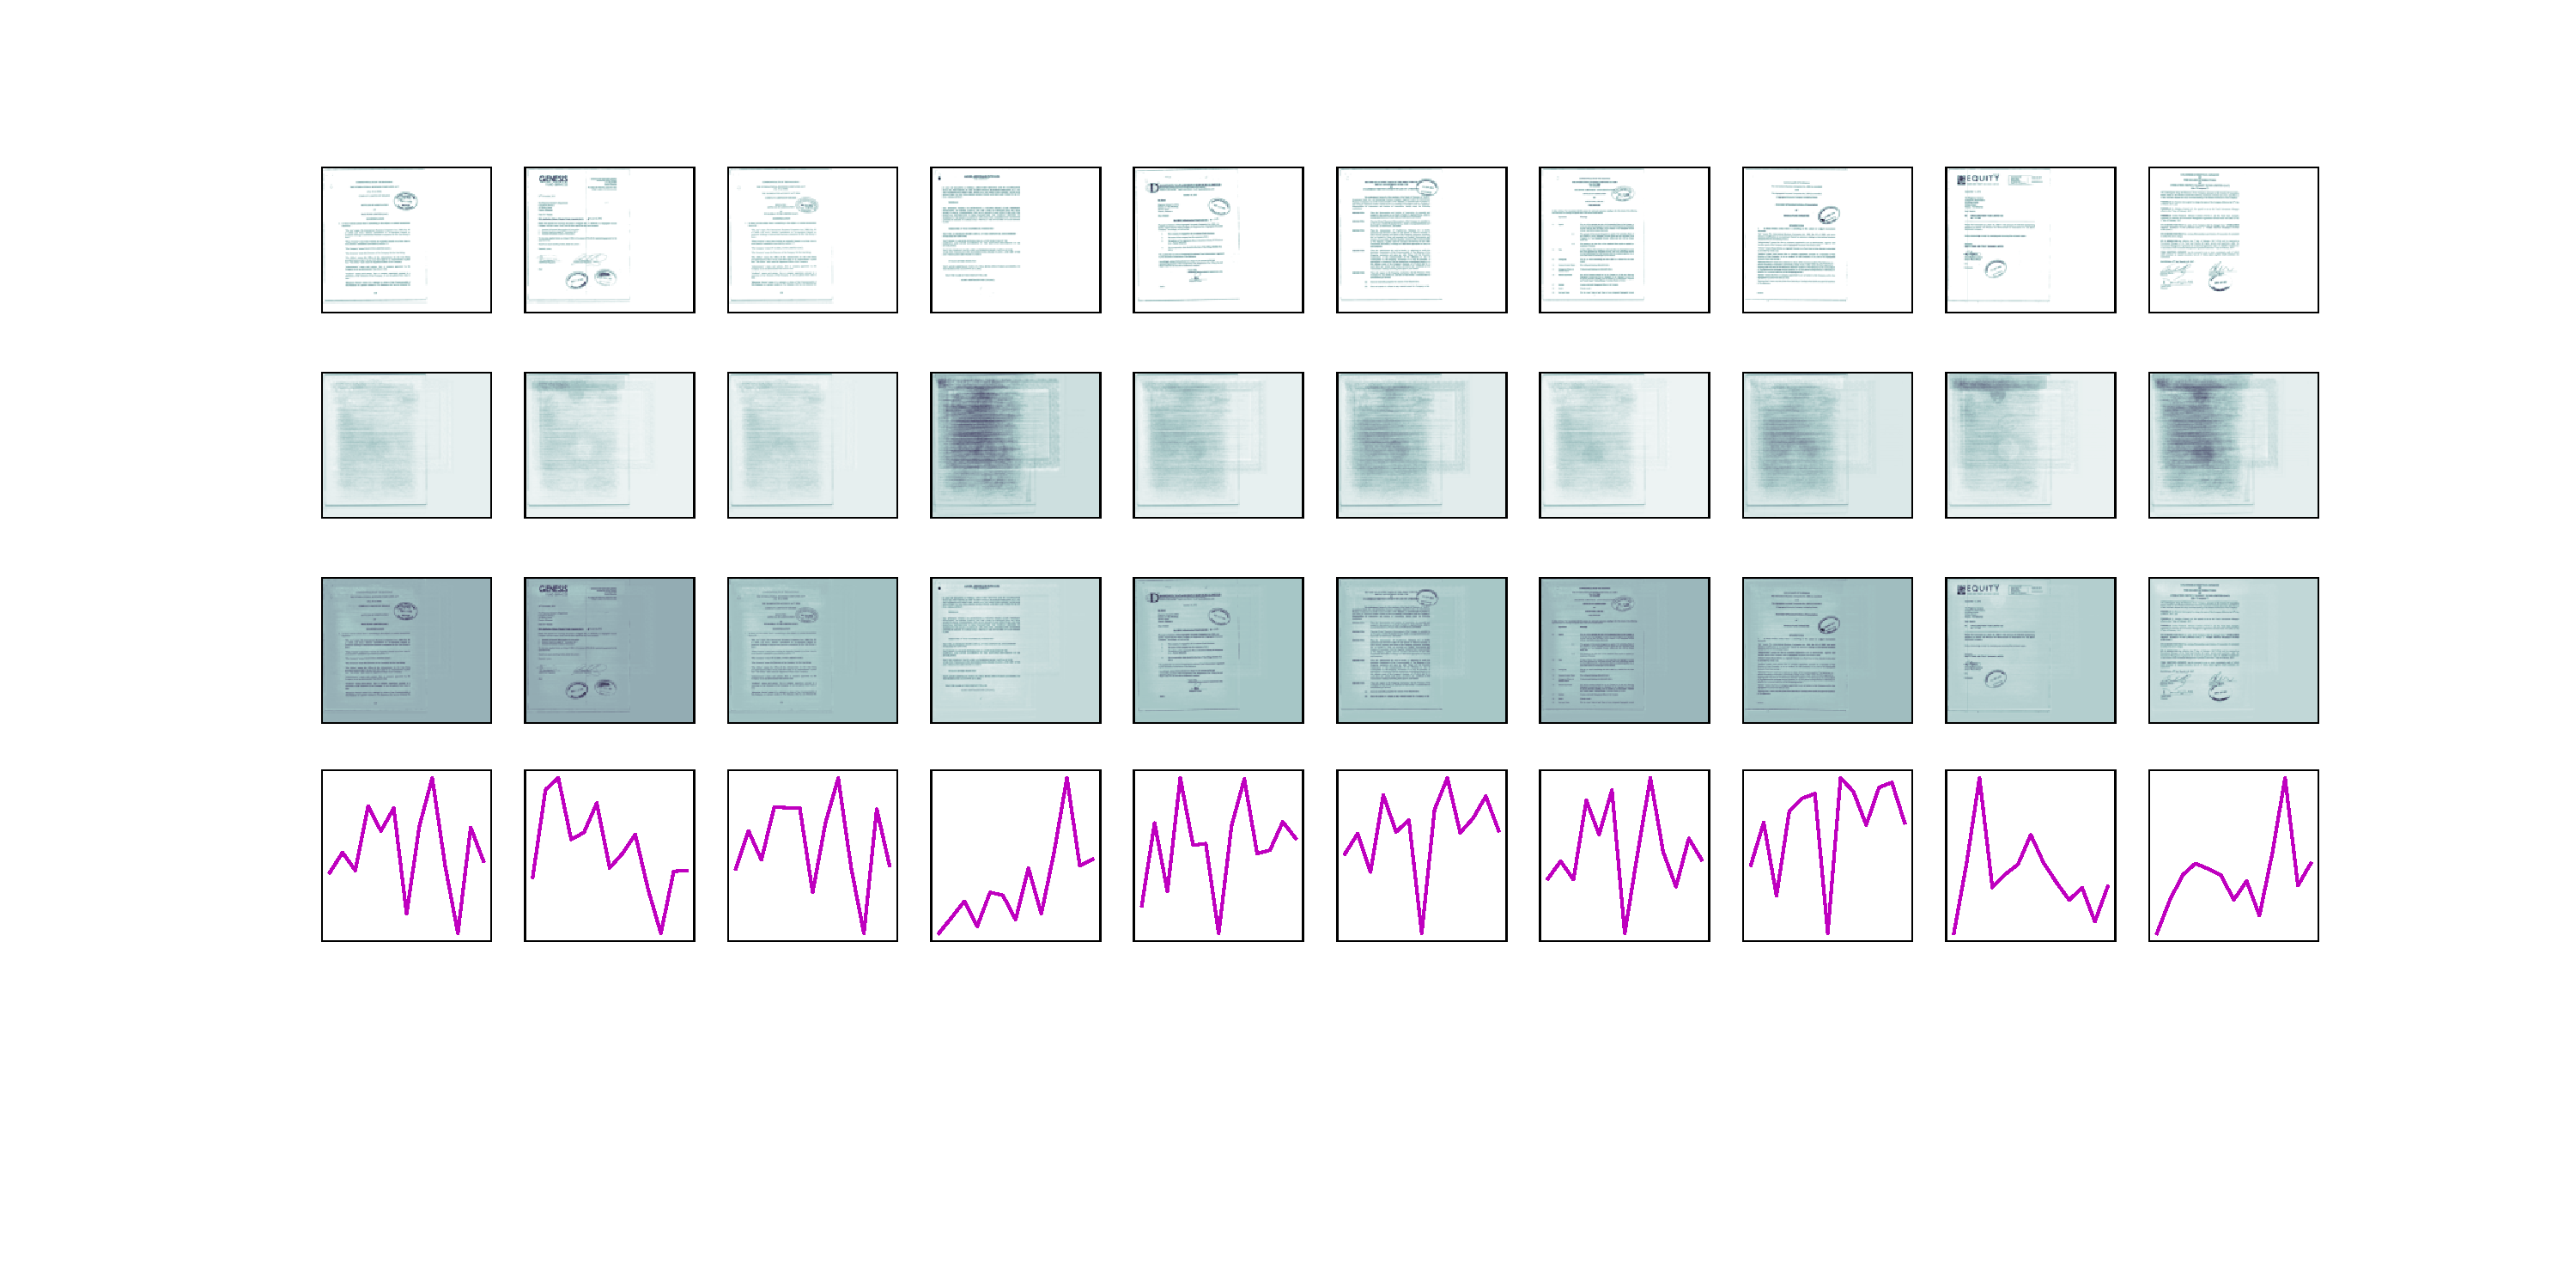
\includegraphics[width=0.7\textwidth]{images/Eigendocs/transformation/eigendocs_13dims.pdf}
    \caption[The first 10 documents of the dataset]{The first 10 preprocessed documents of the dataset.
    The original images are displayed in the first row.
    The second row shows the reconstruction from their compressed version in the fourth row.
    The third row shows the reconstruction error, i.e. the difference between the reconstructed and the original image.
    The last row presents the greyscale values of the compressed 13-dimensional image as a line.
    }
    \label{fig:preprocessed_docs_eigendocs}
\end{figure}

% results
The results of the \eigendocs{} algorithm are displayed in \autoref{fig:preprocessed_docs_eigendocs}.
Assuming that the selection of documents is representative, 
the preprocessing of the documents using \eigendocs{} should have encoded information about the dimensionality of the images.
However, this assumption is not valid since bigger document images exist.
Therefore, the idea of incorporating information about the image's dimensions is not entirely implemented.